\subsection{Notation}
We use the notation \(gh=g\cdot h = g \ast h\) here to represent the group operation (regardless of the specific operation in question).
\subsection{Basic Group Properties}
\begin{proposition}
	Let \(G\) be a group.
	Then,
	\begin{enumerate}[i.]
		\item The identity element \(e\) is unique.
		\item \(\forall g \in G\), the inverse \(g^{-1}\) is unique.
		\item \(g \cdot h = g \iff h \cdot g = g\)
		\item \(g \cdot h = e \iff h \cdot g = e\)
		\item \((gh)^{-1} = h^{-1} g^{-1}\)
		\item \((g^{-1})^{-1} = g\)
	\end{enumerate}
\end{proposition}
\begin{proof}
	We prove each case individually.
	\begin{enumerate}[i.]
		\item Assume \(\exists e, e'\) which are distinct identity elements.
		      We have \(e e' = e\) and \(e e' = e'\) by the definition of the inverse so \(e = e'\) \contradiction{}
		\item Suppose \(h\) and \(k\) are distinct inverses of \(g\).
		      Then \(gh = e\) and \(gk = e\), so:
		      \begin{align*}
			      gh        & = gk                       \\
			      g^{-1} gh & = g^{-1} gk                \\
			      h         & = k \text{ \contradiction}
		      \end{align*}
		\item \begin{align*}
			      gh      & = g  \\
			      \iff gh & = ge \\
			      \iff h  & = e  \\
			      \iff hg & = eg \\
			      \iff hg & = g
		      \end{align*}
		\item \begin{align*}
			      gh              & = e       \\
			      \iff ghg        & = g       \\
			      \iff g^{-1} ghg & = g^{-1}g \\
			      \iff hg         & = e
		      \end{align*}
		\item \((gh) (h^{-1}g^{-1}) = g h h^{-1} g^{-1} = g g^{-1} = e\)
		\item \(g^{-1} g = e\)
	\end{enumerate}
\end{proof}

\begin{definition}[abelian group]
	A group \(G\) is said to be \textit{abelian} if \(\forall a, b, \in G\), \(a \ast b = b \ast a\).
\end{definition}
A common example of an abelian group is the reals under addition.
A non-example is the group of invertible \(2\times 2\) matrices under matrix multiplication.

\begin{definition}
	The order of a group \(G\), denoted \(\abs{G}\), is the number of elements in the set \(G\).
	A group \(G\) is called a finite group if its order is finite, and it is called an infinite group if its order is infinite.
\end{definition}

\subsection{Subgroups}
\begin{definition}
	Let \((G, \ast)\) be a group.
	A subset \(H \subseteq G\) is a subgroup of \(G\) if \((H, \ast)\) is a group.
	We denote this \(H \leq G\).
\end{definition}
We must verify each group axiom on a subset to check if it is a subgroup --- with the notable exception of the associativity axiom, the property of associativity is inherited by subgroups.
Here are some examples of subgroups.

\begin{enumerate}
	\setcounter{enumi}{-1}
	\item \(\{ e \}\) is the trivial subgroup
	\item \(G \leq G\)
	\item \((\mathbb Z, +) \leq (\mathbb Q, +) \leq (\mathbb R, +) \leq (\mathbb C, +)\)
\end{enumerate}
\begin{lemma}
	Let \(G\) be a group.
	\(H \subset G\) is a subgroup of \(G\) if and only if \(H\) is non-empty and \(\forall a, b \in H, ab^{-1} \in H\).
\end{lemma}
\begin{proof}
	We prove each axiom.
	\begin{itemize}
		\item (identity) Setting \(a = b\) gives \(a a^{-1} = e \in H\) as required.
		\item (inverses) Setting \(a = e\), which we know exists from the identity proof above, gives \(b^{-1} \in H\).
		\item (closure) Setting \(b = c^{-1}\), we know that \(c \in H\), and we can always choose a \(b\) such that \(c\) is any value we want; and with the property we can see that \(ac \in H\) as required by the closure axiom.
	\end{itemize}
\end{proof}

\begin{proposition}
	The subgroups of \((\mathbb Z, +)\) are precisely the subsets of the form \(n\mathbb Z \subset Z\) where \(n\mathbb Z := \{nk : k\in \mathbb Z\}\).
\end{proposition}
\begin{proof}
	First, we know that each \(n\mathbb Z\) is a subgroup: given any integer \(n \in \mathbb N\) the axioms hold:
	\begin{itemize}
		\item (closure) given \(nk_1, nk_2 \in n\mathbb Z\), we have \(nk_1 + nk_2 = n(k_1 + k_2) \in n\mathbb Z\)
		\item (identity) \(e = 0 = n \cdot 0 \in n\mathbb Z\)
		\item (inverse) \(-nk = n(-k) \in n\mathbb Z\)
	\end{itemize}
	We also prove the converse statement, namely that the only viable subgroups are of the form \((n\mathbb Z, +)\).
	If \(H = \{ 0 \}\) then clearly \(H = 0\mathbb Z\) which is a trivial subgroup.
	Otherwise, there are some non-zero elements.

	There must be at least one positive element in \(H\), since any negative element can be inverted to make a positive one in \(H\).
	So, let the smallest positive element be \(n\).
	Since \(H\) is a subgroup, it is closed and has inverses.
	This implies that
	\begin{align*}
		n+n+n+\cdots                & \in H; \\
		n^{-1}+n^{-1}+n^{-1}+\cdots & \in H
	\end{align*}
	Therefore \(n\mathbb Z\) is contained within \(H\).
	Now, let us show that there are no extra elements.
	Suppose, for purposes of a contradiction, that \(\exists k \in H \st k \notin n\mathbb Z\).
	Then, since \(k\) is an integer and not a multiple of \(n\), it must lie between two such multiples: \(nm < k < n(m+1)\) where \(m \in \mathbb Z\).
	This means that \(0 < k - nm < n\) which implies that there is a smaller positive element than \(n\) in the set.
	This is a contradiction, so there are no more elements in the set.
\end{proof}

\begin{proposition}
	The following statements are true:
	\begin{itemize}
		\item Let \(H, K\) be subgroups of \(G\).
		      Then \(H \cap K\) is a subgroup of \(G\).
		\item \(K \leq H\) and \(H \leq G\), then \(K \leq G\).
		\item If \(K \subseteq H\), \(H \leq G\) and \(K \leq G\) then \(K \leq H\).
	\end{itemize}
\end{proposition}
% TODO proofs?
% especially for first part

\subsection{Lattice of Subgroups}
We can use a lattice diagram to denote subgroups.
Points below other points joined by lines represent subgroups.
Let \(G, H, K\) be groups and \(H \leq G\) and \(K \leq G\).

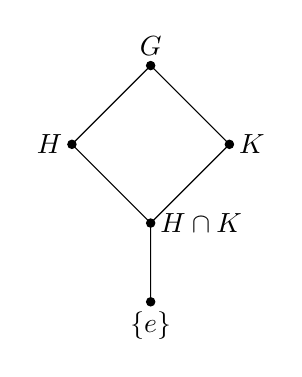
\begin{tikzpicture}
	\draw (0,0) node[below]{\(\{e\}\)}
	-- (0,1) node[right]{\(H \cap K\)}
	-- (1,2) node[right]{\(K\)}
	-- (0,3) node[above]{\(G\)}
	-- (-1,2) node[left]{\(H\)}
	-- (0, 1);
	\filldraw (0,0) circle(1.5pt);
	\filldraw (0,1) circle(1.5pt);
	\filldraw (0,3) circle(1.5pt);
	\filldraw (1,2) circle(1.5pt);
	\filldraw (-1,2) circle(1.5pt);
\end{tikzpicture}

\begin{definition}
	Let \(X \neq \varnothing\) be a subset of a group \(G\).
	The subgroup \textit{generated by} \(X\) denoted \(\genset{X}\) is the intersection of all subgroups containing \(X\).
	Equivalently, \(\genset{X}\) is the smallest subgroup of \(G\) that contains \(X\) as a subset.
	Note that there will always exist some subgroup \(\genset{X}\) regardless of what \(X\) is chosen; a trivial result would be \(G\) itself.
\end{definition}
